%% bulk_genome_properties.tex
%% Author: Leighton Pritchard
%% Copyright: James Hutton Institute
%% A brief description of useful bulk genome properties

% SUBSECTION: Nucleotide frequency and genome size
\subsection{Nucleotide Frequency/Genome Size}

% Calculating GC content/skew
\begin{frame}
  \frametitle{Nucleotide frequency/genome size}
  \begin{itemize}
    \item Very easy to calculate from complete/draft genome
    \item Can calculate for individual contigs/scaffolds/regions
    \item Usually reported in GUI genome browsers
  \end{itemize}    
  Trivial to determine using, e.g. Python
  \begin{center}
    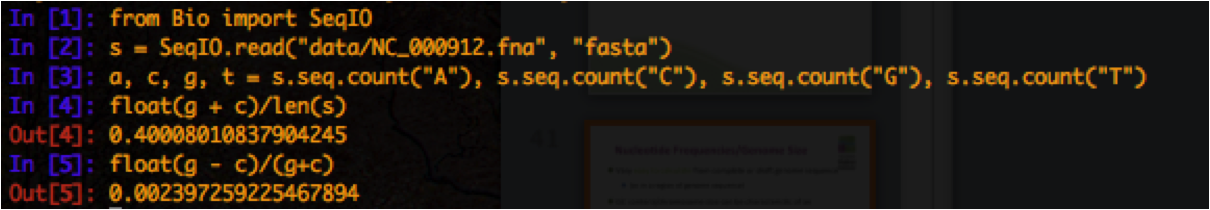
\includegraphics[width=1\textwidth]{images/python_gc}
  \end{center}  
\end{frame}

% GC content and genome size
\begin{frame}
  \frametitle{Nucleotide frequency/genome size}
  GC content and chromosome size can be characteristic\\
  See \texttt{data/bacteria\_size} for example iPython notebook exercise\\[0.5cm]
  \begin{center}
    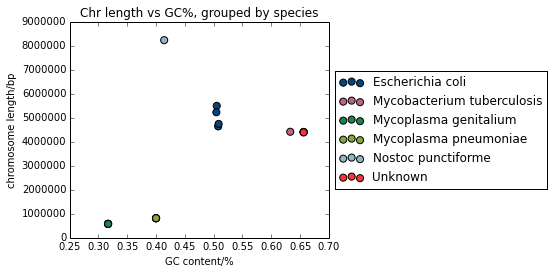
\includegraphics[width=1\textwidth]{images/gc_vs_size}
  \end{center}  
\end{frame}

% Blobology
\begin{frame}
  \frametitle{Blobology\footnote{\tiny{\href{http://dx.doi.org/10.1007/s13199-012-0154-6}{Kumar and Blaxter \textit{et al}. (2011) \textit{Symbiosis} \textbf{3}:119-126 doi:10.1007/s13199-012-0154-6}}}}
  \begin{columns}[T]
    \begin{column}{5cm}
      Sequencing samples may be contaminated or contain microbial symbionts.\\
      Expect more host than symbiont/contaminant DNA\\
      GC content and read coverage can be used to separate contigs, following assembly and mapping\\
      \href{http://nematodes.org/bioinformatics/blobology/}{http://nematodes.org/bioinformatics/blobology/}
    \end{column}
    \begin{column}{5cm}
      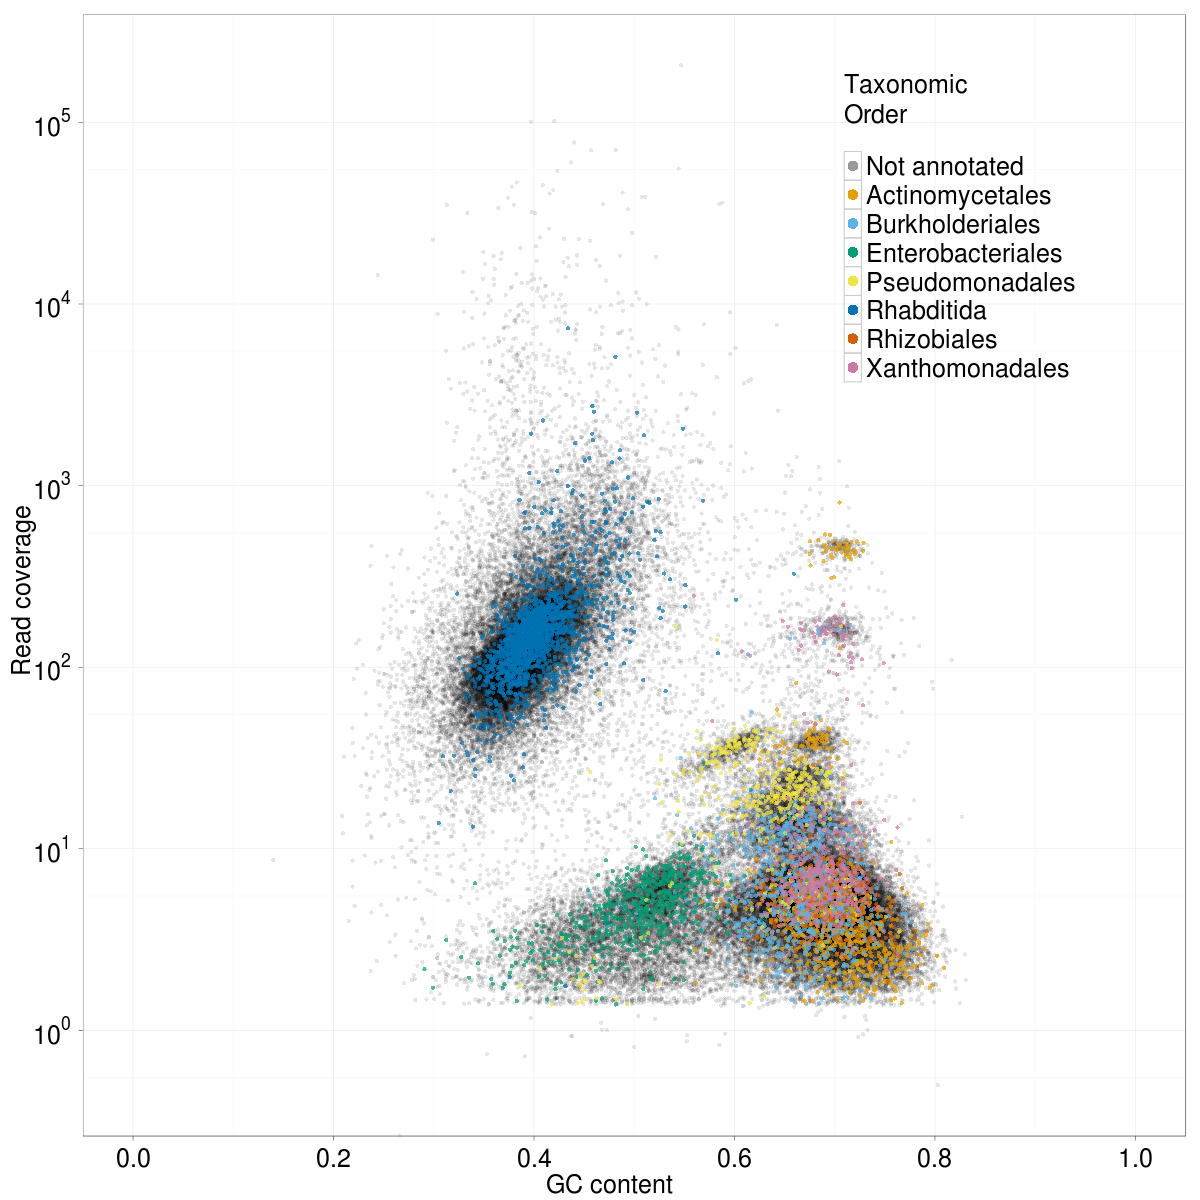
\includegraphics[width=1\textwidth]{images/blobology}
    \end{column}
  \end{columns}
\end{frame}

% k-mers
\begin{frame}
  \frametitle{$k$-mers}
     \begin{itemize}
       \item Nucleotides: \texttt{[ACGT]}
       \item Dinucleotides: \texttt{[AA|AC|AG|AT|CA|CC|$\ldots$]} (16 dimers)
       \item Trinucleotides: 32 trimers
       \item $k$-mers: $4^k$ $k$-mers
     \end{itemize}
     (see example in \texttt{data/shiny})
\end{frame}

% k-mer figures
\begin{frame}
  \frametitle{$k$-mers}
  Diagnostic differences in $k$-mer frequency, and variability.
  \begin{columns}[T]
    \begin{column}{5cm}
    \textit{E.coli}\\
     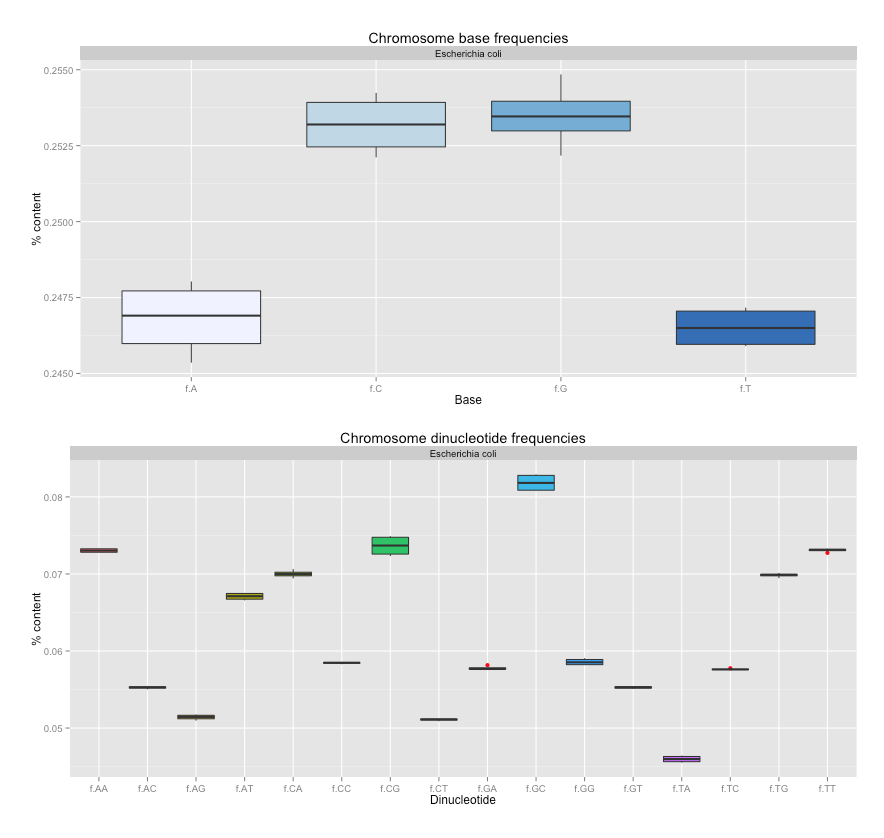
\includegraphics[width=1\textwidth]{images/kmer_ecoli}\\
    \end{column}
    \begin{column}{5cm}     
     \textit{Mycoplasma} spp.
     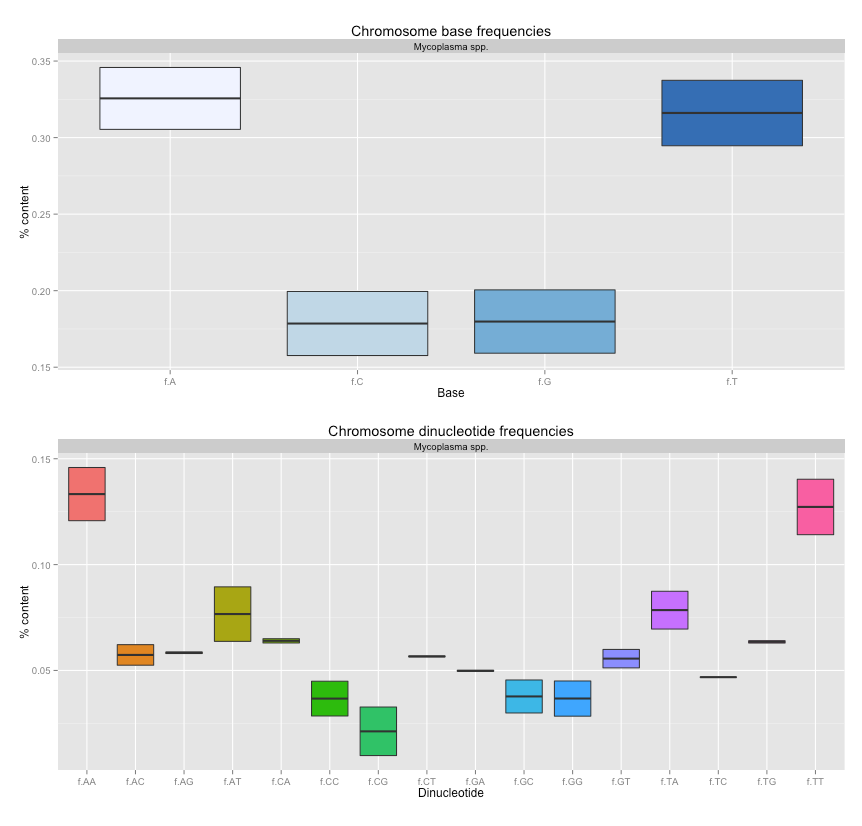
\includegraphics[width=1\textwidth]{images/kmer_mycoplasma}\\
   \end{column}
  \end{columns}
\end{frame}


% SUBSECTION: Nucleotide frequency and genome size
\subsection{Average Nucleotide Identity}

% DNA-DNA hybridisation
\begin{frame}
  \frametitle{DNA-DNA hybridisation\footnote{\tiny{\href{http://dx.doi.org/10.1016/S0168-6445(00)00040-1}{Morello-Mora and Amann (2001) \textit{FEMS Micro. Rev.} \textbf{25}:39-67 doi:10.1016/S0168-6445(00)00040-1}}}}
  \begin{columns}[T]
    \begin{column}{5cm}
      \begin{itemize}
        \item Denature DNA from two organisms.
        \item Allow to anneal. Reassociation $\approx$ similarity, measured as $\Delta T$  of denaturation curves.
        \item Proxy for sequence similarity.
        \item ``Gold Standard'' for prokaryotic taxonomy, since 1960s.
      \end{itemize}
    \end{column}
    \begin{column}{5cm}
      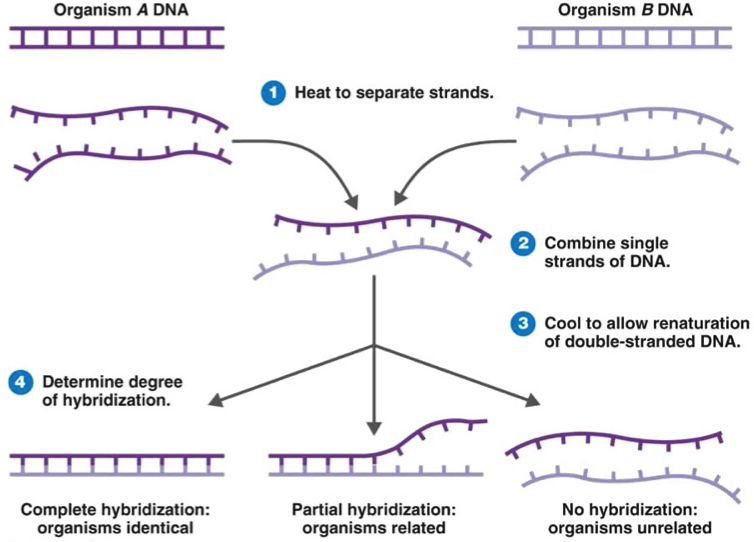
\includegraphics[width=1\textwidth]{images/ddh}
    \end{column}
  \end{columns}
\end{frame}

